\documentclass[30pt, portrait, margin=0mm, innermargin=0mm, blockverticalspace=5mm, colspace=5mm, subcolspace=8mm]{tikzposter}
\geometry{paperheight=24in,paperwidth=36in}
\usepackage{tikz,color,caption,subcaption,hyperref,microtype,graphicx,amsmath,amsthm,amssymb,fixltx2e}
\usepackage[space]{grffile}
\usepackage{graphicx}
\usepackage[utf8]{inputenc}
\usepackage{amsmath}
%\usepackage[table]{xcolor}
\usepackage{tabularx}
\usepackage[backend=bibtex]{biblatex}
\usepackage[colorinlistoftodos,prependcaption,textsize=tiny]{todonotes}

\tikzstyle{line} = [draw, -latex']
\tikzposterlatexaffectionproofoff
\definecolor{trojancardinal}{HTML}{990000}
\definecolor{trojangold}{HTML}{FFCC00}
\usecolorstyle{Default} \usetheme{Simple}
\colorlet{titlebgcolor}{trojancardinal}
\colorlet{blocktitlebgcolor}{trojancardinal}

% Formatting
\setlength{\parskip}{1em}
\renewcommand*{\bibfont}{\footnotesize}

\newcommand{\X}{\cellcolor{blue!25}} 
\newcolumntype{K}[1]{>{\centering\arraybackslash}p{#1}}
\newcolumntype{C}{>{\centering\arraybackslash}X}

\addbibresource{sample.bib}

\interfootnotelinepenalty=10000

\makeatletter
\newcommand\insertlogoi[2][]{\def\@insertlogoi{\includegraphics[#1]{#2}}}
\newcommand\insertlogoii[2][]{\def\@insertlogoii{\includegraphics[#1]{#2}}}
\newlength\LogoSep
\setlength\LogoSep{0pt}

\insertlogoi[width=10cm]{images/SAIL}
\insertlogoii[width=10cm]{images/USC}

\def\title#1{\gdef\@title{\scalebox{\TP@titletextscale}{%
\begin{minipage}[t]{\linewidth}
\centering
#1
\par
\vspace{0.5em}
\end{minipage}%
}}}

\renewcommand\maketitle[1][]{  % #1 keys
    \normalsize
    \setkeys{title}{#1}
    % Title dummy to get title height
    \node[transparent,inner sep=\TP@titleinnersep, line width=\TP@titlelinewidth, anchor=north, minimum width=\TP@visibletextwidth-2\TP@titleinnersep]
        (TP@title) at ($(0, 0.5\textheight-\TP@titletotopverticalspace)$) {\parbox{\TP@titlewidth-2\TP@titleinnersep}{\TP@maketitle}};
    \draw let \p1 = ($(TP@title.north)-(TP@title.south)$) in node {
        \setlength{\TP@titleheight}{\y1}
        \setlength{\titleheight}{\y1}
        \global\TP@titleheight=\TP@titleheight
        \global\titleheight=\titleheight
    };

    % Compute title position
    \setlength{\titleposleft}{-0.5\titlewidth}
    \setlength{\titleposright}{\titleposleft+\titlewidth}
    \setlength{\titlepostop}{0.5\textheight-\TP@titletotopverticalspace}
    \setlength{\titleposbottom}{\titlepostop-\titleheight}

    % Title style (background)
    \TP@titlestyle

    % Title node
    \node[inner sep=\TP@titleinnersep, line width=\TP@titlelinewidth, anchor=north, minimum width=\TP@visibletextwidth-2\TP@titleinnersep]
        at (0,0.5\textheight-\TP@titletotopverticalspace)
        (title)
        {\parbox{\TP@titlewidth-2\TP@titleinnersep}{\TP@maketitle}};

    \node[inner sep=0pt,anchor=west] 
      at ([xshift=-\LogoSep]title.west)
      {\@insertlogoi};

    \node[inner sep=0pt,anchor=east] 
      at ([xshift=\LogoSep]title.east)
      {\@insertlogoii};

    % Settings for blocks
    \normalsize
    \setlength{\TP@blocktop}{\titleposbottom-\TP@titletoblockverticalspace}
}
\makeatother

\title{\fontfamily{put}\selectfont \textcolor{trojangold}{\textbf{Continuous Real-time Annotation Fusion via Rank-based Signal Warping}}}
\author{\textcolor{trojangold}{\textbf{\Large{Brandon M. Booth$^\dagger$, Karel Mundnich$^\ddagger$, Shrikanth S. Narayanan$^\ddagger$}}}}
\institute{\vspace{-0.1in}\textcolor{trojangold}{\large $^\dagger$Department of Computer Science, $^\ddagger$Department of Electrical Engineering}}

\begin{document}

\maketitle[width=0.65\textwidth, titletotopverticalspace=18pt, titletoblockverticalspace=18pt, titlegraphictotitleverticalspace=18pt]

\begin{columns}

\column{0.25}

\block{Motivation}{
\setlength{\parindent}{3em}
\noindent
{\Large \textbf{Continuous human annotations are noisy} and prone to unintended influence from personal bias, task ambiguity, environmental distractions, and more.  \textbf{Can we remove these artifacts?} \\ \\}
{\Large Try this annotation challenge:}
\begin{tikzfigure}
	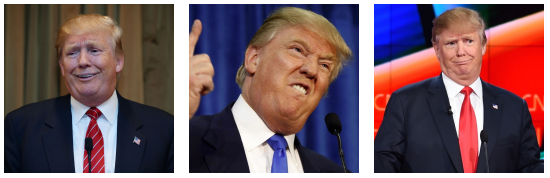
\includegraphics[width=0.18\textwidth]{images/GoofyFaces}
	{\Large How goofy are these faces on a [0,1] scale?}
\end{tikzfigure}
\vspace{25pt}
\noindent
{\Large Why is this hard?  Goofiness does not have an intuitive scale.  Now try to find which two faces are more similar.\\ \\}
{\Large \textbf{People are better at ranking than rating.} \cite{yannakakis2015ratings}}
}

\block{Our Approach}{
\setlength{\parindent}{3em}
\noindent
\begin{itemize}
\item Propose \textbf{rank-based signal warping} to complement existing annotation fusion methods
\item \textbf{Validate on experiment} with an objective truth
\end{itemize}
}

\column{0.25}

\block{Experiment}{
\setlength{\parindent}{3em}
\noindent
Ten annotators rate the intensity of the color green in a video in real-time.
\begin{tikzfigure}[]
	\centering
	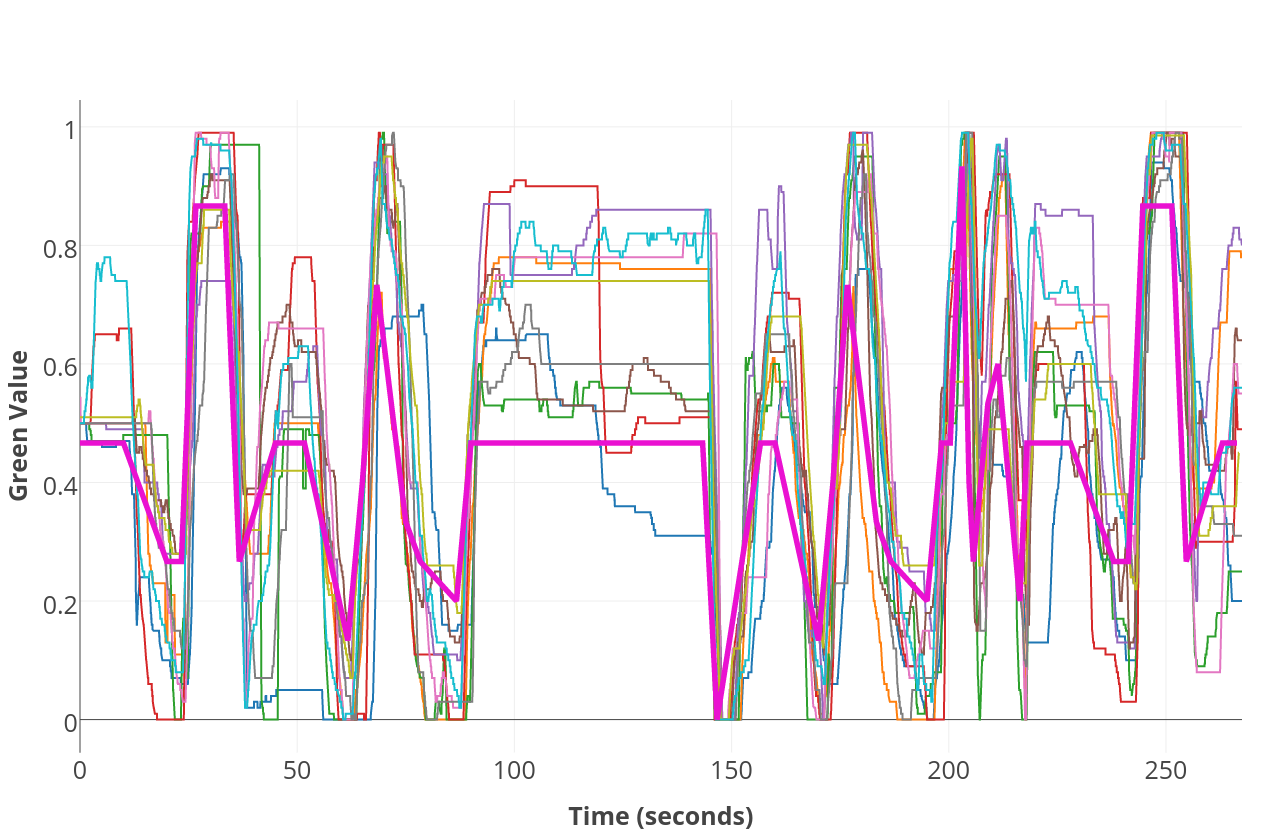
\includegraphics[width=0.20\textwidth]{images/annotations_ot}
	Annotations alongside the true value (\textbf{bold})
\end{tikzfigure}
\vspace{25pt}
Annotators \textbf{cannot capture trends while preserving self-consistency}.
}

\block{Rank-based Warping}{
\setlength{\parindent}{3em}
\noindent
\begin{enumerate}
\item Apply any state-of-the-art annotation fusion method
\item Extract nearly constant intervals using total variation denoising \cite{becker2011templates}
\item Collect additional annotations comparing triplets of constant intervals
\item Construct ordinal embedding from constant intervals (using t-STE) \cite{van2012stochastic}
\item Warp signal to align with embedding (Figure 1)
\end{enumerate}
}

\column{0.5}

\block{}{
\centering
{\uppercase \normalsize Agreement measures for baseline and warped fused annotation approaches \\ \\ }
\vspace{25pt}
\begin{tabular}{ |c|c|c|c|c| } 
 \hline
 Signal Type & Pearson & Spearman & Kendal's Tau & NMI \\ 
 \hline
 Simple Average & 0.775 & 0.795 & 0.636 & 0.302 \\ 
 Warped Average & \textbf{0.811}$^\dagger$ & 0.738 & 0.584 & 0.307 \\
 \hline
 EvalDep Average & 0.906 & 0.946 & 0.830 & 0.484 \\
 Warped EvalDep & \textbf{0.967}$^\dagger$ & 0.939 & 0.835 & 0.562 \\
 \hline
\end{tabular}
\vspace*{18pt} \\
{\footnotesize A $^\dagger$ denotes significant improvement ($p < 0.005$, Fisher z-transform).  Warped results use a complete set of ordinal comparisons. NMI = normalized mutual information.}

\setcounter{figure}{0}
\begin{tikzfigure}
\normalsize
\begin{IEEEeqnarray}{}
S_t &=& 
\begin{cases}
\mathcal{E}_i - \frac{1}{|\mathcal{I}_i|}\sum\limits_{s \in \mathcal{I}_i} y_{s} & \exists \mathcal{I}_i \in \mathcal{I} : t \subseteq \mathcal{I}_i \\
0 & o.w.
\end{cases} \\
y_t' &=& 
\begin{cases}
y_t + S_t & \exists \mathcal{I}_i \in \mathcal{I} : t \subseteq \mathcal{I}_i \\
\Big(\frac{y_t-y_a}{y_b-y_a}\Big)(y_b + \mathcal{S}_{b^+}) + \Big(\frac{y_b-y_t}{y_b-y_a}\Big)(y_a + y'_{a^-}) & \exists [a,b] = \mathcal{J}_j \in \mathcal{J} : t \subseteq \mathcal{J}_j
\end{cases}
\end{IEEEeqnarray} \\
\vspace{4pt}
{\small Fig. 1: Let $\mathcal{I}$, $\mathcal{J}$ and $\mathcal{E}$ be the ordered sets of intervals, inter-intervals and embedding values.  Let $t \in \{1,2,...,T\}$, $y_t$ denote the fused annotation, and $y'_t$ denote the warped signal value. Subscript $+$ or $-$ denote a time just before or after the time index.}
\end{tikzfigure}
}

\begin{subcolumns}

\subcolumn{0.5}

\block{Results}{
\setlength{\parindent}{3em}
\noindent
\begin{tikzfigure}[]
	\centering
	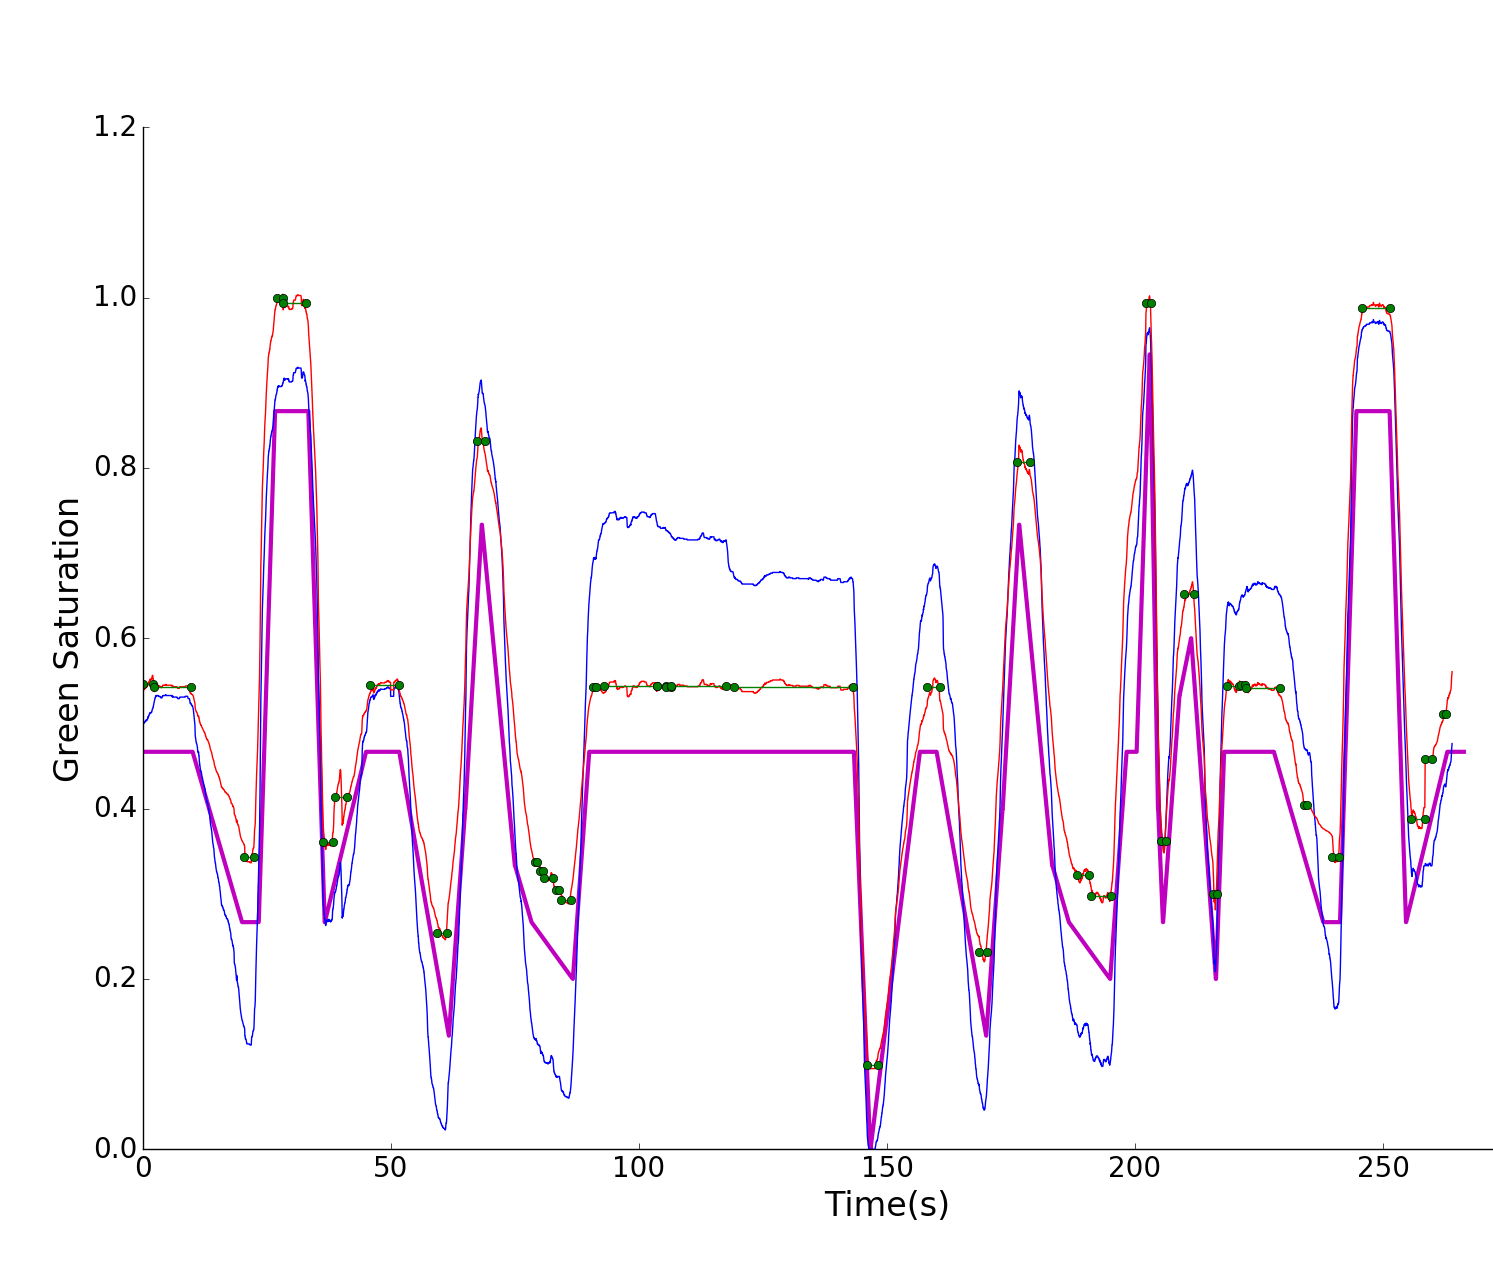
\includegraphics[width=0.19\textwidth]{images/warp_evaldep}
	\textbf{Objective truth (magenta), fused annotations (blue), warped signal (red), embedded intervals (green)}
\end{tikzfigure}
}

\subcolumn{0.5}

\block{Conclusion}{
\setlength{\parindent}{3em}
\noindent
{\Large We leverage the \textbf{natural ability of human annotators to annotate trends} in real-time and \\ \\}
{\Large \textbf{We separately leverage accurate similarity comparisons} to achieve accurate ground truth.}
{\printbibliography}
}

\end{subcolumns}

\end{columns}

\end{document}